%\chapter{Lesson 13.03.2020} % 13 marzo 2020
\section{Hedging}\lesson{3}{13/03/2020}
We saw that the price of a given payoff is given by \eqref{fig:fc_payoff}, so we solved the problem of pricing. This completely solve the problem for the long position, who wants to know which is the correct price to pay to the short position in order to get the payoff at the end. \\
Now we have to solve the problem for the short position. One possibility is to sell the option (possibility) and hope that the market goes in the right direction, but this it is not a good strategy. For the short position we have to build up a portfolio which value at time $T$ is exactly the payoff we have to give to the long position. This problem is known as \emph{hedging}. The strategy is the following:
\begin{enumerate}
    \item Solve the pricing problem
    \item Take $\alpha$ shares, i.e. the number of shares that we have to hold in our portfolio in order to replicate the payoff:
    \begin{equation}
        \alpha = \dfrac{f^u-f^d}{Su-Sd} =  \dfrac{\Delta\mbox{payoff}}{\Delta S} \equiv \Delta
    \end{equation}
    This quantity is know in general as \emph{delta} and it represents the amount of underlying we have to get in the portfolio in order to replicate the payoff of the option.
    \item Invest into the riskless market, taking $\beta$ according to \eqref{V0}:
    \begin{equation}
        \beta = price_0-\Delta S_0
    \end{equation}
\end{enumerate}
\begin{example}{}{}
Consider again the toy model where we have an underlying which initial price is $S_0=100$, $T=1$ year, $S_T=(Su,Sd)=(110,90)$, a strike price $K=100$ and an interest rate of $1\%$ per year. Then we have
\begin{equation*}
    u = \dfrac{110}{100} = 1.1 \qquad d = \dfrac{90}{100} = 0.9
\end{equation*}
The corrisponding $q$ is
\begin{equation*}
    q = \dfrac{e^{RT}-d}{u-d} = \dfrac{e^{0.01}-0.9}{1.1-0.9} = 0.555
\end{equation*}
Now we are able to compute the price of the call:
\begin{equation}
    price_0(\mbox{call}) = e^{-RT}(10q+ 0(1-q)) = 10qe^{-RT} = 5.44
\end{equation}
This is the market price coherent with the no arbitrage principle of a promise that can give a payoff between 10 and 0. So, in order to use the replicating portfolio strategy, the short position has to sell the option for a price $\mbox{price}^{mkt}>5.44$. The income of $\mbox{price}^{mkt}-5.44$ can be put in the pocket, but we have to use 5.44 in order to build up the hedging strategy, which consists in taking
\begin{equation*}
    \Delta = \dfrac{f^u-f^d}{Su-Sd} = \dfrac{10-0}{110-90} = 0.5
\end{equation*}
shares in the risky market and
\begin{equation*}
    \beta = price_0-\Delta S_0 = 5.44 - 0.5\cdot100 = -44.56
\end{equation*}
For example, if the underlying is worth \EUR{100}, I have to invest \EUR{50} in the risky market. But if we are in the short position we don't have \EUR{50}, because we receive only \EUR{5.44} from the long position. So we take the \EUR{5.44} and we borrow \EUR{44.56} from the riskless market in order to invest in the risky market\footnote{In the real market you don't buy one $\Delta = 0.5$ but you consider a package of two options and the global hedging.}. \\
In this kind of business we usually get slightly more than price$_0$. For example, if price$_0$ = \EUR{5.44} we would expect to get something like \EUR{5.54}. Notice that for a personal business of \EUR{0.10} we are obliged to construct a trading strategy which involves an investment of \EUR{50} in the risky market and \EUR{44.56} in the riskless market, so we have to move a huge amount of money compared to what we get at the end. That's why it is very important to be precise in the hedging strategy.
\end{example}

\section{Dividends}
A \emph{dividend} is a payment made by a corporation to its shareholders. The idea is that if we own one asset sometimes the corresponding corporate decides to give us -- in addition to the market value of our asset -- some extra bonus. \\
Consider a binomial model in which we have and underlying with initial value $S$ and final values given by the terminal values $Su,Sd$ plus a bonus:
\begin{equation}
    S \to \begin{cases}
    Su + Se^{\delta T} \\ Sd + Se^{\delta T}
    \end{cases}
\end{equation}
where $\delta$ is called \emph{dividend rate} and in general is a random variable. In such cases we say that the price is \emph{cum dividend}, whereas if there is no dividend the price is \emph{ex dividend}. We can repeat the same arguments we did before for the price ex dividend introducing the dividend as a shift of the price of the underlying. The probability weight becomes
\begin{equation}
    q = \dfrac{e^{RT}-(d+e^{\delta T})}{u-d}
\end{equation}
\begin{remark}
    Recall that in Remark \ref{remark} we found a stylized case of martingale. Now we have
    \begin{equation}
        \mathbb{E}^{\Qmeas}[S_T] = S_0(e^{RT}-e^{\delta T})
    \end{equation}
    so it is not true anymore that discounted assets are constant in expected value.
\end{remark}

\subsection{Put-call parity}\label{putcallparity}
One interesting thing is that it is possible to deduce the implicit dividend policy of a corporate -- which usually is private -- from the prices quoted in the market. In order to do that we use the \emph{put-call parity}, which is a link between the put and the call prices. \\
Start by considering no dividends. Notice that any number can be written as positive part minus negative part:
\begin{equation*}
    x = x^+ - x^- = x^+ - (-x)^+
\end{equation*}
So, we can write
\begin{equation}
    S_T - K = \underbrace{(S_T - K)^+}_{call} - \underbrace{(K - S_T)^+}_{put}
\end{equation}
Now we use the linearity of expected value:
\begin{equation*}
    \mathbb{E}^{\Qmeas}[S_T-K] = \mathbb{E}^{\Qmeas}[(S_T-K)^+] - \mathbb{E}^{\Qmeas}[(K-S_T)^+]
\end{equation*}
and multiply both sides for the discounted value:
\begin{equation*}
    e^{-RT}\mathbb{E}^{\Qmeas}[S_T-K] = \underbrace{e^{-RT}\mathbb{E}^{\Qmeas}[(S_T-K)^+]}_{call_0} -
    \underbrace{e^{-RT}\mathbb{E}^{\Qmeas}[(K-S_T)^+]}_{put_0}
\end{equation*}
where we recognized the initial price of the call and of the put. Then we use the property ${\mathbb{E}}[aX+b]=a{\mathbb{E}}[X]+b$:
\begin{equation*}
    e^{-RT}\mathbb{E}^{\Qmeas}[S_T-K] = e^{-RT}\mathbb{E}^{\Qmeas}[S_T] - Ke^{-RT} = \mathbb{E}^{\Qmeas}[e^{-RT}S_T] - Ke^{-RT} \overset{\eqref{S0}}{=} S_0 - Ke^{-RT}
\end{equation*}
In the end, we get:
\begin{equation}\label{put-call}
    S_0 - Ke^{-RT} = call_0 - put_0 \qquad\Rightarrow\qquad put_0 = call_0 - S_0 +  Ke^{-RT}
\end{equation}
Now consider the presence of dividends the put-call parity becomes
\begin{equation}\label{put-call-div}
    put_0 = call_0 - S_0 +  Ke^{-RT} + S_0e^{(\delta - R)T}
\end{equation}
that means that if for the same asset there is a market of put options and call options with a certain maturity, then we consider the list of the quoted prices of the put and of the call and use eq. \eqref{put-call-div} to find $\delta$.

\section{Market completeness}
Let's consider the following assumptions:
\begin{enumerate}
    \item short positions and fractional holdings of the underlying are allowed;
    \item there is no \emph{bid-ask spread}, i.e. there is no difference between the prices quoted for an immediate sale (ask) and an immediate purchase (bid) for an underlying;
    \item there are no transaction costs;
    \item there is a perfectly liquid market, i.e. there is the possibility to buy or sell an unlimited quantity of an underlying.
\end{enumerate}
\begin{definition}[Reachable contingent claim]
    A contingent claim\footnote{A contingent claim is a derivative whose future payoff depends on the value of another “underlying” asset, or more generally, that is dependent on the realization of some uncertain future event.} $x\in\mathbb{R}^2$ is \emph{reachable} if there exists a portfolio $h(\alpha,\beta)$ with terminal value $V^h_T=x$ almost surely (i.e. with probability 1). In this case $h$ is called hedging portfolio.
\end{definition}
\begin{definition}[Complete market]
    If all the claims are reachable, the market is \emph{complete}.
\end{definition}
So, in a complete market it is possible to replicate all the possible random variables, i.e. all the possible contracts.
\begin{proposition}\label{prop1}
    If a claim $x$ is reachable with $h$ and there is absence of arbitrage opportunity, then the price of $x$ is
    \begin{equation}
        price_0(x) = V_0^h.
    \end{equation}
\end{proposition}
\begin{remark}
    If a claim $x$ is reachable than Prop. \ref{prop1} holds also in an incomplete market.
\end{remark}
\begin{proposition}\label{prop2}
    The binomial model with $d<e^{RT}<u$ is arbitrary free and complete.
\end{proposition}
\noindent So, in a static binomial model it is possible to price everything. The next step is to consider a dynamic model.

\section{The multi period case}
We want to generalize the binomial model
\begin{equation*}
    S\to\begin{cases}
    Su \\ Sd
    \end{cases}
\end{equation*}
For example we can introduce a third possible realization of the underlying, obtaining a trinomial model:
\begin{equation*}
    S\to\begin{cases}
    Su \\ Sm \\ Sd
    \end{cases}
\end{equation*}
In this case, since we have only two tools in our investment strategy (the risky and rikless markets) if, for example, we want to replicate a call option, the payoff is
\begin{equation*}
    (S_T-K)^+ = \left(\begin{matrix}
        (Su-K)^+ \\ (Sm-K)^+ \\ (Sd-K)^+
    \end{matrix}\right)
\end{equation*}
and we have to solve three equations with two unknowns, which -- apart from special cases -- is impossible to solve. So, just adding one more possible outcome leads to uncomfortable consequences in terms of pricing methodology, because our model is no more complete. We have the possibility to invest in the risky market and in the riskless market in order to follow the fluctuations of something which can take three values, so the underlying fluctuates too much. We need another instrument to follow the flutuations of the underlying, for example an extra underlying $S'$, but things become complicated. It is much more convenient to introduce a dynamic framework. For example, consider the following tree.
\begin{center}
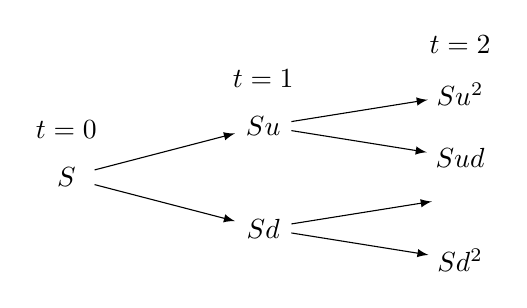
\begin{tikzpicture}[
                   grow = right,
edge from parent/.style = {draw,-latex},
         label distance = 1.5mm,
      every node/.style = {minimum width=2em, inner sep=3pt},
         level distance = 25mm,
       sibling distance = 10mm,
                     ]
\node[label=90:{$t=0$}] {$S$}
    child {node {$Sd$}
        child {node {$Sd^2$}
            %child {node {40}}
            %child {node {20}}
                }
        child {node {}}%<---------------- already printed
            }
    child {node[label=90:{$t=1$}] {$Su$}
        child {node {$Sud$}
            %child {node {}}%<------------ already printed
            %child {node {0}}
                }
        child {node[label=90:{$t=2$}] {$Su^2$}
            %child {node {}}%<------------ already printed
            %child {node[label=90:{$t=3$}] {0}}
                }
                };
\end{tikzpicture}
\end{center}
In this case the tree is stationary, i.e. $u$ and $d$ are always the same for every $t$. This tree is called \emph{recombining tree} or \emph{lattice}. Computationally speaking this is an advantage because if we have $n$ steps then the terminal values are $n+1$, so the number of all the possible realizations remains linear with respect to time.\\
Conversely, if we consider a non-recombining tree, like
\begin{center}
\tikzstyle{level 1}=[level distance=25mm, sibling distance=13mm]
\tikzstyle{level 2}=[level distance=25mm, sibling distance=8mm]
\begin{tikzpicture}[grow=right,->,>=angle 60]
  \node {$S$}
    child {node {$Sd_1$}
      child {node {$Sd_1d_2$}
      }
      child {node{$Sd_1u_2$}
      }
    }
    child {node {$Su_1$}
      child {node{$Su_1d_2$}
      }
      child {node{$Su_1u_2$}
      }
    };
\end{tikzpicture}
\end{center}
for $n$ steps we have $2^n$ possible realizations, which for large $n$ is impossible to manage.\\
The decision between combining and non-combining tree is crucial, and it should be motivated by some financial argument. Why should we use non-recombining trees? What we observe in the market is that when $S$ goes up the volatility is low, whereas when the market decreases there is an increase of the volatility.
\begin{figure}[h]
    \centering
    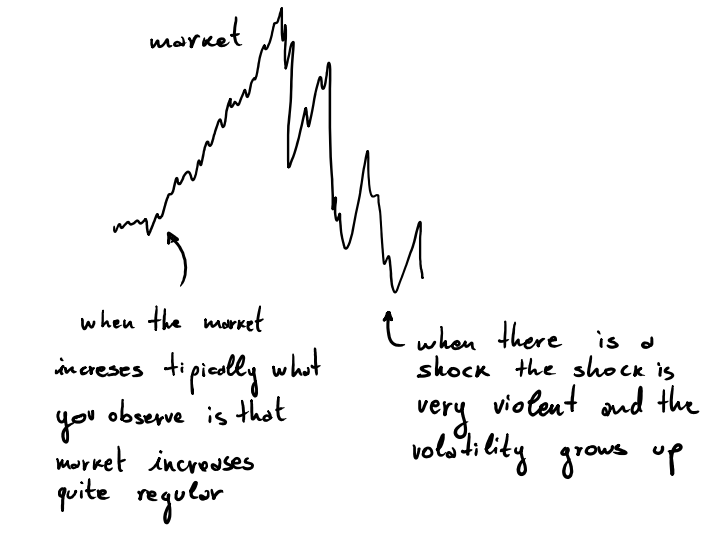
\includegraphics[scale=0.2]{fig/tmp/fig6}
    \caption{Volatility behavior.}
    \label{fig:figura6}
\end{figure}
This is the reason why it could be interesting to consider a non-recombining tree. However, if we choose this kind of model there is a problem in the implementation. Recall that in the binomial model $u$ and $d$ are given by $(u,d)\sim e^{\pm\sigma\sqrt{T}}$: the problem is we have only one historical series, and if the parameters vary step by steps it is impossible to estimate them. So we drop this model and we use a recombining tree.
\begin{remark}
    Sometimes it is not possible to use a recombining tree because there are same contracts which payoff depends on the whole past history of the underlying. So, in these cases it is not enough to take a picture of the underlying at the maturity. For example, in the 70s some manipulations have been used in order to rise the price of crude oil immediately before the maturity and then exercise the call option, buying at $K<S_T$ and getting $S_T-K>0$. In order to avoid this kind of manipulations, contracts which payoff depends on the whole past history of the underlying -- called \emph{asian options} -- have been introduced. Asian options payoff is given by
    \begin{equation}
        \mbox{payoff}_T = \left(\dfrac{1}{T}\int^T_0 S_s\,ds-K\right)^+
    \end{equation}
\end{remark}
